\documentclass{beamer}
\usepackage[utf8]{inputenc}
\usepackage[T1]{fontenc}

\usebackgroundtemplate{
	
\includegraphics[width=\paperwidth,height=\paperheight]{img/background}
}

\title{Chapter 01: Structured Analysis}

\author[P.A. Nugroho]{Pascal Alfadian Nugroho}
\institute[IF-UNPAR]{Program Studi Informatika, \\Universitas Katolik Parahyangan}

\begin{document}
	\begin{frame}
		\titlepage
	\end{frame}
	
	\section{Specification Document}
	\subsection{Overview}
	\begin{frame}{Specification Document}
		\begin{itemize}
			\item Contract between client and developer
			\item Specifies precisely what the product must do and constraints of the product
			\item Almost always, includes deadline
			\item Includes set of acceptance criteria
			\item \textbf{Does not} specify how the product is made unless specifically needed
			\item There can be many ways in writing a specification document
		\end{itemize}
	\end{frame}
	\subsection{Example}
	\begin{frame}{Specification Document: Example}
		\begin{center}
			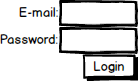
\includegraphics[scale=0.5]{img/01_login}
		\end{center}
		\begin{enumerate}
			\item The login screen must show two inputs: email and password
			\item Password must be transmitted securely to server using HTTPS
			\item The error message for ``unregistered user'' and ``invalid password`` must be exactly the same
			\item \textit{The login screen must be implemented using HTML5 and CSS3 standard} % example of requirement that specifically governs how the product is made
		\end{enumerate}
	\end{frame}
	\subsection{Goals}
	\begin{frame}{Specification Document: Goals}
		\begin{itemize}
			\item Agreement between client/user and development team
			\item Let development team fully understands the problem
			\item Hence a \textit{solution strategy}(-ies) can be suggested
		\end{itemize}
	\end{frame}

	\section{Informal Specifications}
	\subsection{Overview}
	\begin{frame}{Informal Specifications}
		Example of informal specification using \textit{natural language} \cite[page 462]{Schach:2006:OCS:1207045}:
		\begin{quotation}
		BV.4.2.5. If the sales for the current month are below the target sales, then a report is to be printed, unless the difference between target sales and actual sales is less than half of the difference between target sales and actual sales in the previous month or if the difference between target sales and actual sales for the current month is under 5 percent.
	\end{quotation}
	\end{frame}
	\subsection{Problems}
	\begin{frame}{Informal Specifications: Problems}
		\begin{itemize}
			\item Lengthy sentence to explain accurately what the product should behave
			\item Ambiguous, e.g. when comparing to last month, is it in terms of percentage or in dollars?
		\end{itemize}
	\end{frame}	

	\section{Structured Analysis}
	\subsection{Overview}
	\begin{frame}{Structured Analysis}
		\begin{columns}[t,totalwidth=\textwidth]
			\column{.5\linewidth}
				\begin{itemize}
					\item A more formal way of specification
					\item Use of graphics for specification was an important technique in 1970s (until today)
					\item Several techniques become popular, but we will use \cite{gane1977structured} as suggested in main reference
					\item That is, a nine-step technique (summary on the right, explained in detail later)
				\end{itemize}
			\column{.5\linewidth}
			\begin{flushright}
				\small{
					\begin{enumerate}
						\item Draw the \textbf{Data Flow Diagram} (DFD) of existing system
						\item Decide what sections to computerize and how
						\item Determine the details of the data flows
						\item Define the logic of the process
						\item Define the data source
						\item Define the physical resources
						\item Determine the input-output specifications
						\item Perform the sizing
						\item Determine the hardware requirements
					\end{enumerate}
				}
			\end{flushright}
		\end{columns}		
	\end{frame}
	\subsection{Case Study: Sally's Software Show}
	\begin{frame}{Case Study: Sally's Software Show}
		\begin{itemize}
			\item Buys software from various suppliers and sells it to public
			\item Monthly turnover of 300 packages
			\item Average retail cost of \$250 each
			\item Analysis:
			\begin{itemize}
				\item Which parts should be computerized?
				\item What's the objective to computerize?
				\item Assumption: Sally wishes to computerize ``to make more money''
			\end{itemize}
		\end{itemize}
	\end{frame}
	\subsection{Step 1: Draw The DFD}
	\begin{frame}{Step 1: Draw The DFD}
		\begin{center}
			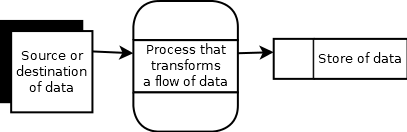
\includegraphics[scale=0.5]{img/01_dfd_symbols}
		\end{center}	
		\begin{itemize}
			\item A pictorial representation of all aspects of the logical data flow
			\item Constructed by identifying the \textbf{data flows}
			\item Each flow of data starts and ends either at
			\begin{itemize}
				\item \textbf{Source or destination of data} (double-square box) or
				\item \textbf{Data store} (open-ended rectangle)
			\end{itemize}
			\item Data are transformed by one or more \textbf{process}es (rounded rectangle)
		\end{itemize}
	\end{frame}
	\begin{frame}{Step 1: Draw The DFD}
		\begin{columns}[t,totalwidth=\textwidth]
			\column{.5\linewidth}
				\begin{itemize}
					\item DFD is generally large, therefore need to be developed in stepwise refinement
					\item Above is example for Sally's Software Shop, first refinement
					\item That diagram can have many intepretations
					\item See two possible implementation in next slide
				\end{itemize}			
			\column{.5\linewidth}
				\begin{flushright}
					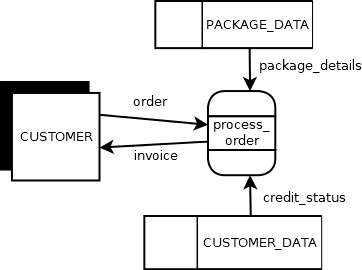
\includegraphics[scale=0.5]{img/01_sally_dfd_first_refinement}
				\end{flushright}
		\end{columns}		
	\end{frame}
	
	\section{References}
	\begin{frame}[allowframebreaks]
	        \frametitle{References}
	        \bibliographystyle{amsalpha}
	        \bibliography{module_01}
	\end{frame}
\end{document}

